\documentclass{article}
\usepackage[utf8]{inputenc}
\usepackage{graphicx}
\usepackage{hyperref}
\hypersetup{
    colorlinks=true,
    linkcolor=blue,
    filecolor=magenta,
    urlcolor=cyan,
}

\urlstyle{same}

\begin{document}

\title{COVID-19 Victims Database Project}
\author{Livxy}
\date{March 2023}

\maketitle
% add some indents so the title is on the top of the page
\thispagestyle{empty}
\vspace{50cm}


\section{Introduction}
The COVID-19 pandemic has affected the world in many ways. \
The pandemic has caused many deaths and has affected the economy. \
We can use data to understand the impact of the pandemic on the world. \
The COVID-19 victims database project is a project that collects and analyzes data related to COVID-19 victims.

\begin{figure}[h]
\centering
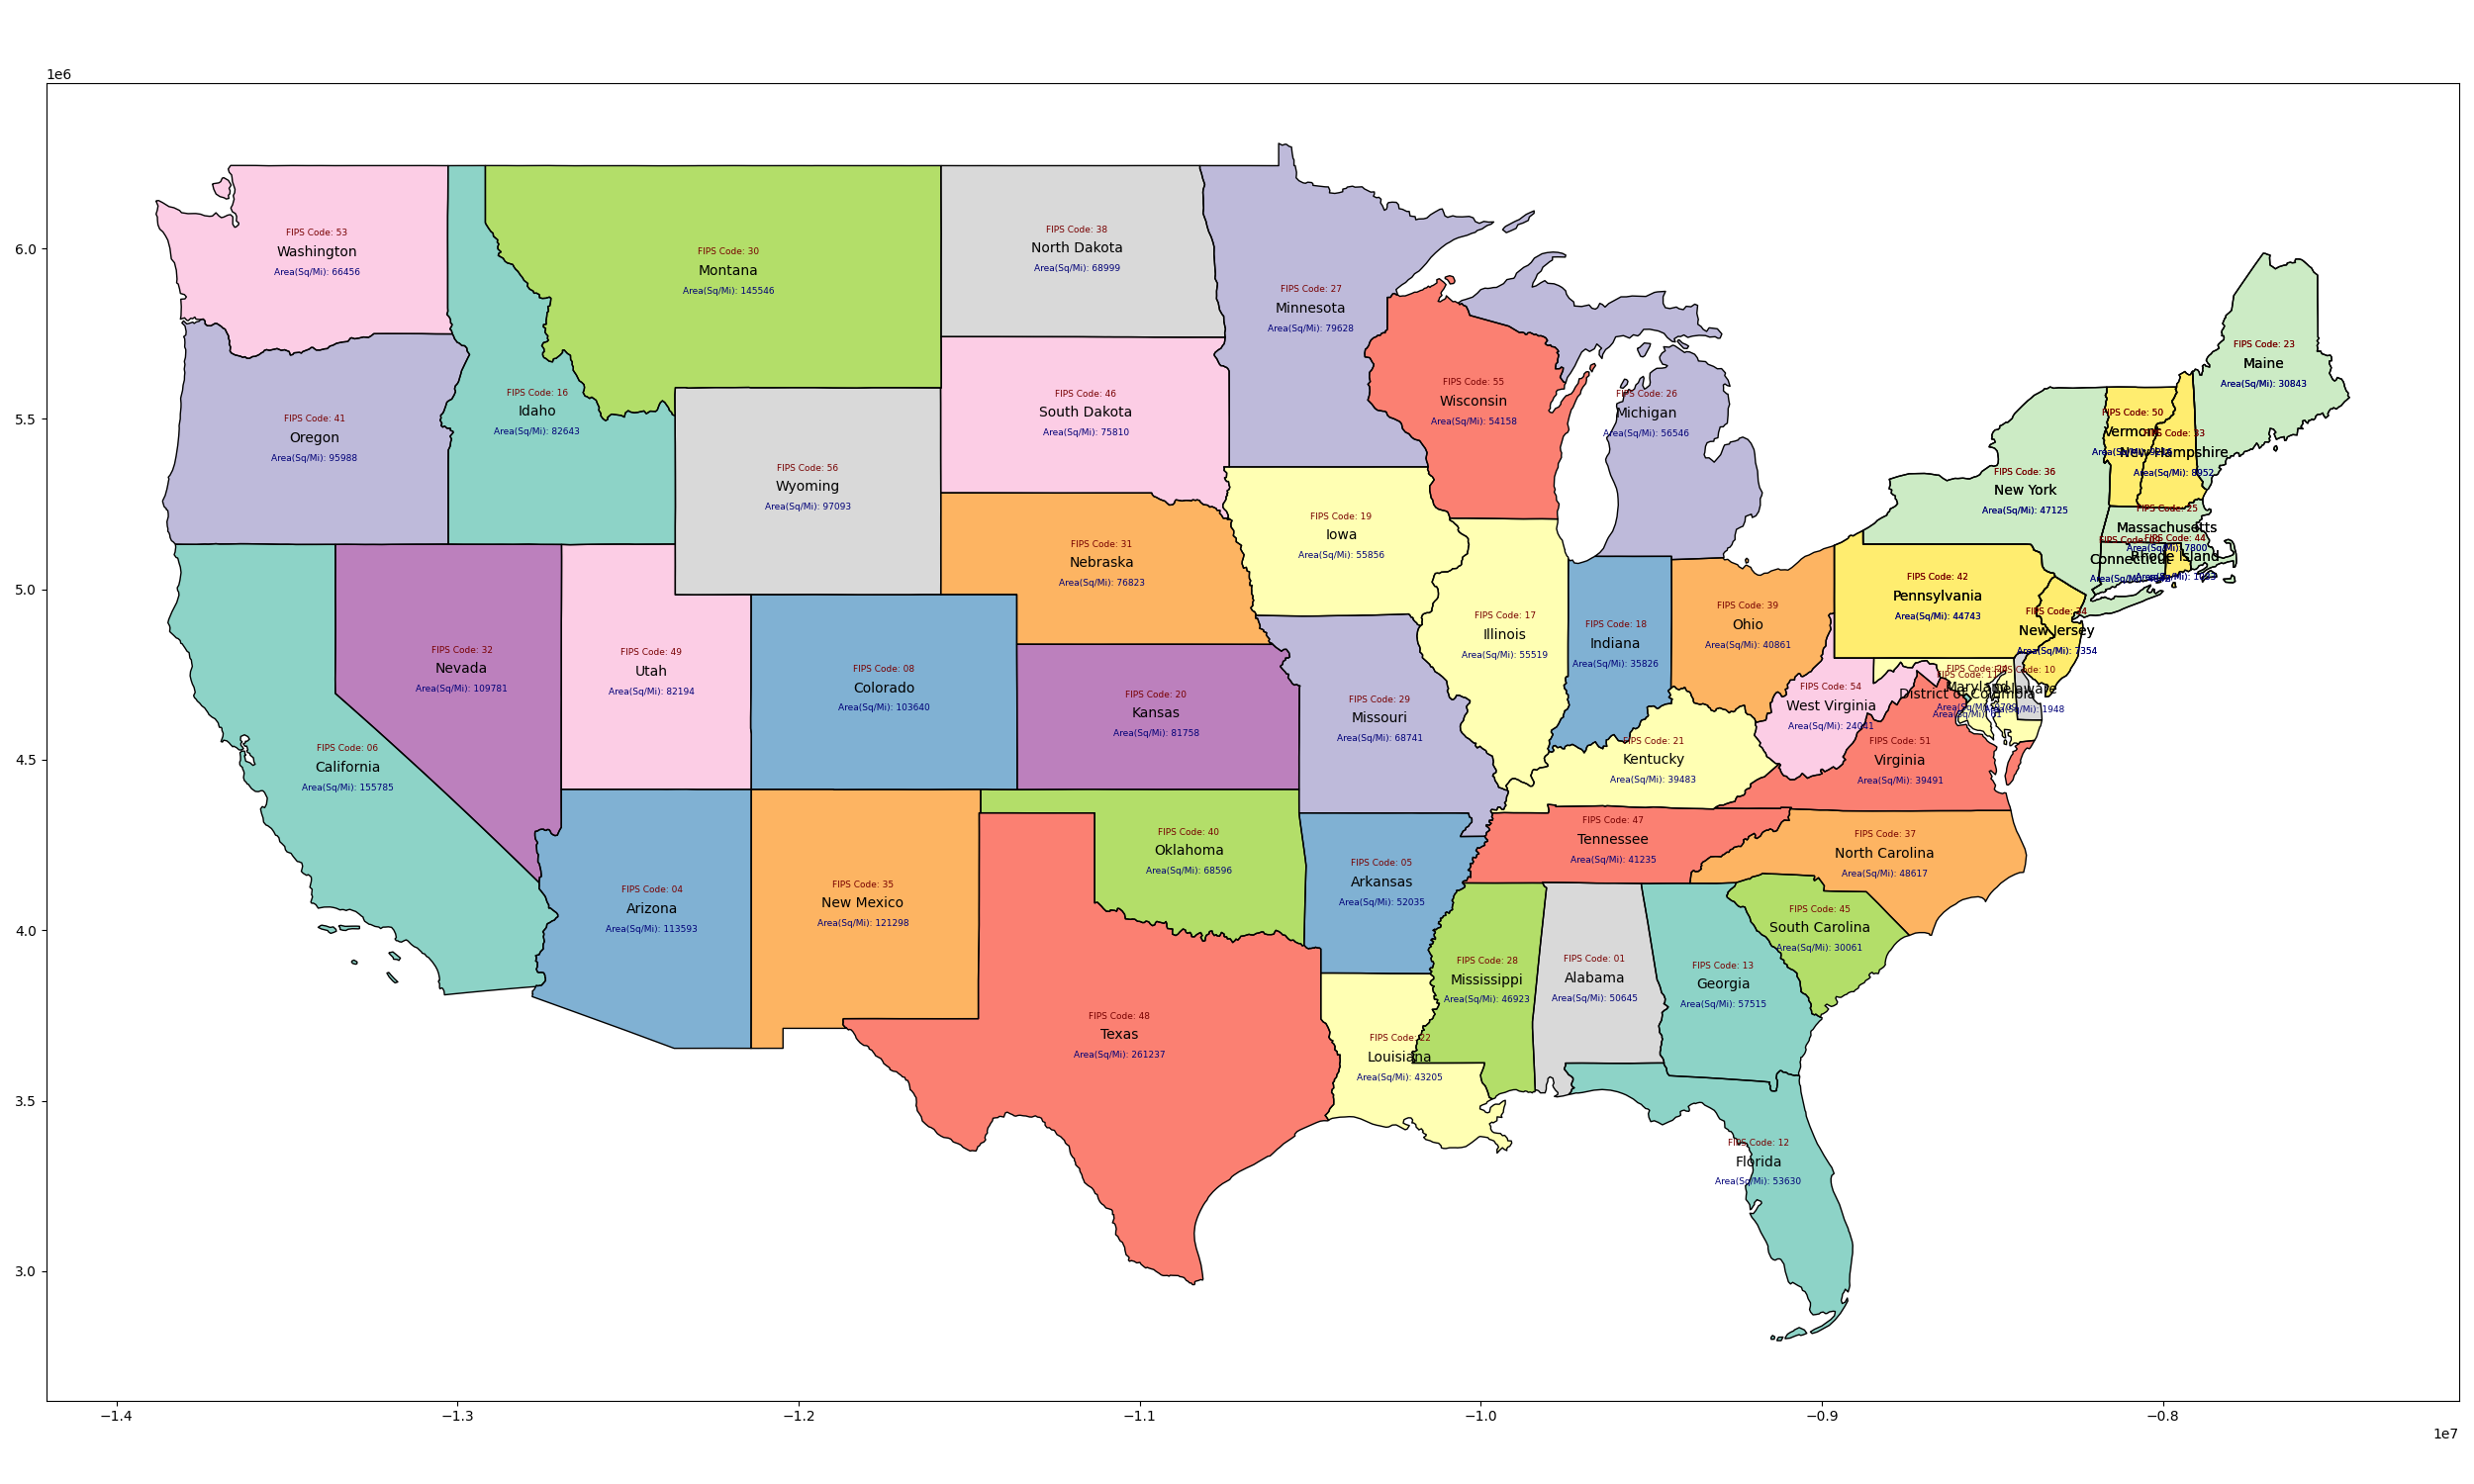
\includegraphics[width=1\textwidth]{images/USA.png}
% \caption{COVID-19 victims in the US}
\end{figure}


\section{Data Collection}
The data collection process is automated using Python. \
The data is collected from the following sources: \
\begin{itemize}
\item \url{https://www.worldometers.info/coronavirus/}
\item \url{https://www.cdc.gov/coronavirus/2019-ncov/cases-updates/summary.html}
\item \url{https://github.com/joncutrer/geopandas-tutorial/tree/master/data}
\item \url{https://github.com/nytimes/covid-19-data}
\end{itemize}



\section{Survivability Analysis}


\section{Visualization}

\section{Conclusion}
The COVID-19 victims database project is an important project that can help us understand the impact of the COVID-19 pandemic on the world. \
By collecting and analyzing data related to COVID-19 victims, we can gain insights into the survivability of having COVID-19 and contacting it. \
The project can also help us identify high-risk groups and take measures to protect them. \
By using Python to automate the data collection and analysis process, we can save time and resources and focus on the analysis and interpretation of the data.

\section{Credit}
% give thank you to https://github.com/joncutrer/geopandas-tutorial/tree/master/data for the map data
Thank you to Jon Cutrer for providing the map data. \
The map data is available at \url{https://github.com/joncutrer/geopandas-tutorial/tree/master/data}.
\\\\
Thank you to the New York Times for providing the COVID-19 data. \
The COVID-19 data is available at \url{https://github.com/nytimes/covid-19-data}.

\end{document}